\begin{figure}[H]
\centering
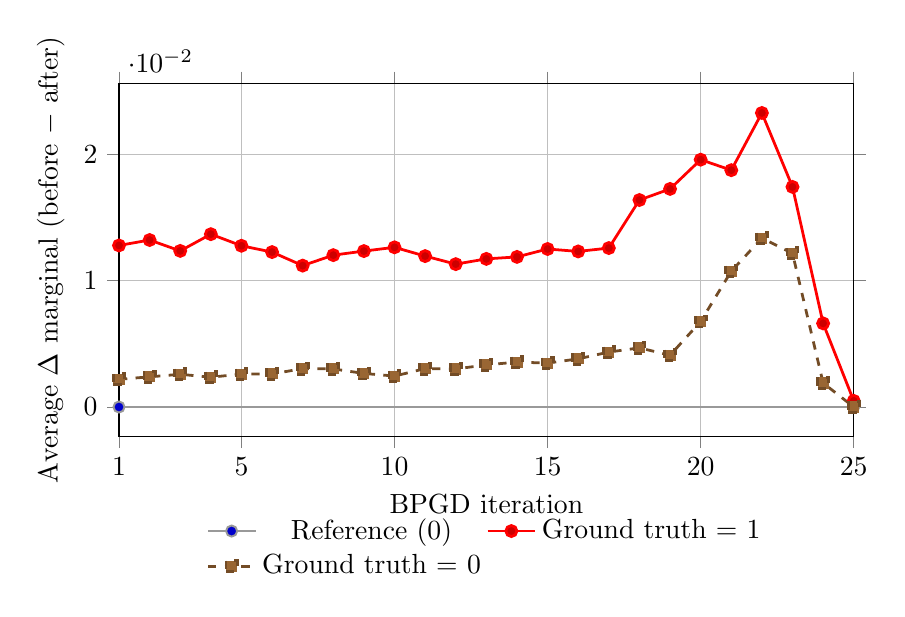
\begin{tikzpicture}
\begin{axis}[
  width=0.9\linewidth, height=0.5\linewidth,
  xlabel={BPGD iteration},
  ylabel={Average $\Delta$ marginal (before $-$ after)},
  xmin=1, xmax=25,
  xtick={1,5,10,15,20,25},
  ymajorgrids, grid=both,
  tick align=outside,
  legend columns=2,
  legend style={at={(0.5,-0.2)},anchor=north,draw=none,fill=none},
  % Uncomment next two lines if you prefer "improvement-positive" for GT=1:
  % yticklabel style={/pgf/number format/fixed},
  % y label style={align=center},
]
  % Zero reference
  \addplot+[smooth, domain=1:25, samples=2, line width=0.7pt, color=black!40] {0};
  \addlegendentry{Reference (0)}

  % === GT = 1 curve (your first vector) ===
  \addplot+[
    mark=*,
    line width=1pt,
  ] coordinates {
    (1, 0.01277997) (2, 0.01321043) (3, 0.01234875) (4, 0.01367217) (5, 0.01275521)
    (6, 0.01225579) (7, 0.01118489) (8, 0.01201370) (9, 0.01233569) (10, 0.01263245)
    (11, 0.01193830) (12, 0.01130253) (13, 0.01171802) (14, 0.01187442) (15, 0.01250025)
    (16, 0.01230669) (17, 0.01257457) (18, 0.01637567) (19, 0.01725165) (20, 0.01956591)
    (21, 0.01873445) (22, 0.02326167) (23, 0.01741204) (24, 0.00661565) (25, 0.00048573)
  };
  \addlegendentry{Ground truth = 1}

  % === GT = 0 curve (your second vector) ===
  \addplot+[
    mark=square*,
    dashed,
    line width=1pt,
  ] coordinates {
    (1, 0.00219178) (2, 0.00238550) (3, 0.00258879) (4, 0.00235593) (5, 0.00260759)
    (6, 0.00261363) (7, 0.00303784) (8, 0.00301133) (9, 0.00265429) (10, 0.00244694)
    (11, 0.00303629) (12, 0.00300891) (13, 0.00333170) (14, 0.00355504) (15, 0.00347144)
    (16, 0.00380908) (17, 0.00434687) (18, 0.00467745) (19, 0.00409546) (20, 0.00676624)
    (21, 0.01074063) (22, 0.01335998) (23, 0.01215781) (24, 0.00189862) (25, 0.00000000)
  };
  \addlegendentry{Ground truth = 0}
\end{axis}
\end{tikzpicture}
\caption{Average per-step change in marginals when clamping evidence during BPGD.
Positive values mean the marginal decreased after the update (since $\Delta=\text{before}-\text{after}$).
Curves are averaged over the test set.}
\label{fig:bpgd_delta_marginals}
\end{figure}